\documentclass{article}

\usepackage{latexsym}
\usepackage[empty]{fullpage}
\usepackage{titlesec}
\usepackage{marvosym}
\usepackage[usenames,dvipsnames]{xcolor}
\usepackage{verbatim}
\usepackage{enumitem}
\usepackage[pdftex]{hyperref}
\usepackage{fancyhdr}
\usepackage{fontawesome5}
\usepackage{pifont}
\usepackage{tabularx}
\usepackage{graphicx}
\usepackage{xcolor}
\hypersetup{
    colorlinks,
    linkcolor={red!50!black},
    citecolor={blue!50!black},
    urlcolor={blue!80!black}
}

\pagestyle{fancy}
\fancyhf{} % clear all header and footer fields
\fancyfoot{}
\renewcommand{\headrulewidth}{0pt}
\renewcommand{\footrulewidth}{0pt}

% Adjust margins
\addtolength{\oddsidemargin}{-0.530in}
\addtolength{\evensidemargin}{-0.375in}
\addtolength{\textwidth}{1in}
\addtolength{\topmargin}{-.45in}
\addtolength{\textheight}{1in}

\urlstyle{rm}

\newcommand{\jobTitle}[3]{
\vspace{0.4cm}
\begin{tabularx}{0.99\linewidth}{ X r }
    \textbf{#1} & #2\\
    \textit{#3} &
\end{tabularx}
\vspace{0.2cm}
}

\titleformat{\section}{
  \scshape\raggedright\large
}{}{0em}{}[\color{RoyalPurple}\titlerule\vspace{-0.4cm}]
\setlength\parindent{0em}

\renewcommand{\labelitemi}{\textcolor{RoyalPurple}{\ding{111}}}
\renewcommand{\labelitemii}{\textcolor{RoyalPurple}{--}}
\newenvironment{descitemize}
{ \begin{itemize}[leftmargin=1.4cm,,topsep=0pt]
    \setlength{\parskip}{0pt}
    \setlength{\parsep}{0pt}     }
{ \end{itemize}                  } 

\begin{document}
\setlength{\footskip}{3.60004pt}
\textbf{\LARGE Lemuel LEE Kwok Lam}
\vspace{0.15cm}

Computer Science Penultimate Year Student
\vspace{0.3cm}

\begin{tabular}{@{} l @{\space}l | l @{\space}l | l }
    \faEnvelope &\href{mailto:lemuellee.kl@gmail.com}{lemuellee.kl@gmail.com} &
    +44 & 07597 243 186 &
    London
    \\
    \faGlobe &\href{https://lemuellee.com}{lemuellee.com} & +852 & 6238 2237 & Hong Kong\\
    \faLinkedin & \href{https://linkedin.com/in/lemuelkl}{linkedin.com/in/lemuelkl}\\
    \faGithub & \href{https://www.github.com/LemuelKL}{github.com/LemuelKL}
\end{tabular}

\vspace{0.5cm}
\hfill
\smash{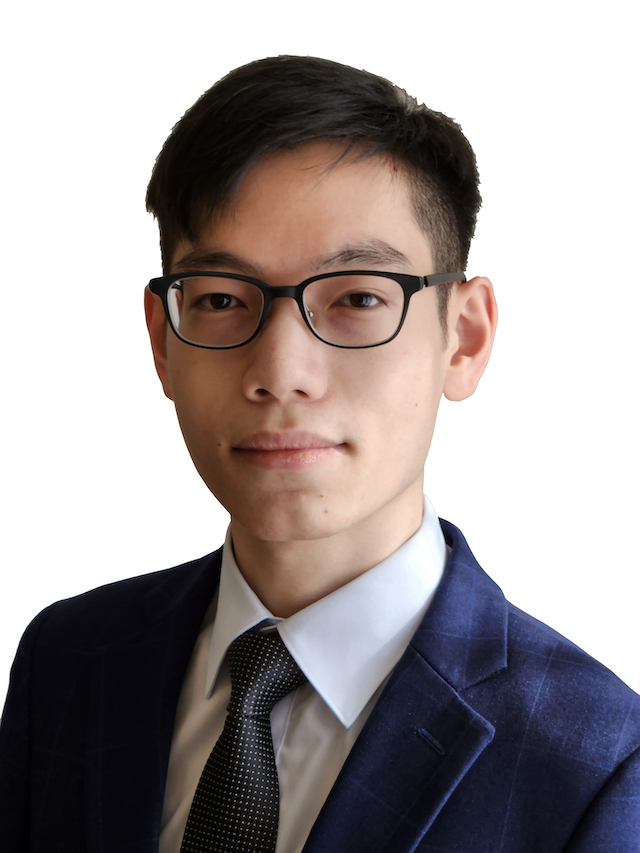
\includegraphics[width=3cm]{avatar-white-small.jpg}}

\vspace{-0.3cm}
\section{EXPERIENCE}

\jobTitle
{Question Writer \& Programmer}
{Mar 2021 --- Aug 2021 \& Jul 2022 --- Aug 2022 }
{Shatin Pui Ying College}
\begin{descitemize}
    \item Authored multiple-choice question templates following the HKDSE Mathematics and Physics syllabuses
    \item Developed and programmed in a custom external domain-specific language based on JavaScript and KaTeX
    \item Used such language to generate HTML code, mathematical tables, graphs, and 3D graphics
    \item Typeset mathematical equations
    \item Featured on Sing Tao Daily: \href{https://std.stheadline.com/smartparents/article/2572}{https://std.stheadline.com/smartparents/article/2572}
\end{descitemize}

\jobTitle
{Full Stack Developer}
{Jun 2022 --- Aug 2022}
{Shatin Pui Ying College}
\begin{descitemize}
    \item Developed an electronic ticketing system for the school Musical
    \begin{itemize}
        \item Semi-automated order management, seat arrangement, mission control, and bulk e-mailing
        \item Real-time multi-user editing with different permission levels
    \end{itemize}
    \item Developed a series of timetable scheduling web apps for exams, lessons, and HKDSE invigilation
    \begin{itemize}
        \item Supports multiple constraints such as teacher availability, room capacity, and lesson duration
    \end{itemize}
\end{descitemize}

\jobTitle
{Student Teaching Assistant}
{Sep 2021 --- Dec 2021 \& Jan 2022 --- Jun 2022}
{The University of Hong Kong}
\begin{descitemize}
    \item ENGG1340 Computer Programming II: Advanced Python programming, Linux shell commands, Shell scripts, C/C++ programming, Separate compilation techniques
    \item ENGG1330 Computer Programming I: Python programming, Searching and sorting algorithms
    \item Hosted weekly lab sessions
    \item Reviewed assignments according to a marking scheme and gave individual video feedback
\end{descitemize}

\section{EDUCATION}

\jobTitle
{Bachelor of Engineering in Computer Science}
{Sep 2020 --- Jun 2024}
{The University of Hong Kong}
\begin{descitemize}
    \item Pursuing Focus --- Theoretical Computer Science
\end{descitemize}

\jobTitle
{International Exchange}
{Jan 2023 --- Jun 2023}
{Royal Holloway, University of London}
\begin{descitemize}
    \item Computer Science
\end{descitemize}

\jobTitle
{Secondary Education --- Hong Kong Diploma of Secondary Education}
{Sep 2013 --- Jun 2020}
{Shatin Pui Ying College}
\begin{descitemize}
    \item First in Information and Communications Technology in final year
    \item Third in Physics in final year
\end{descitemize}

\vspace{3cm}
\section{CERTIFICATIONS}

\jobTitle
{IELTS Academic}
{May 2022}
{Overall 7.5}

\jobTitle
{Hong Kong Diploma of Secondary Education}
{2020}
{Chinese, English, Mathematics, Liberal Studies, Information and Communications Technology, Physics}

\jobTitle
{TOEIC Listening \& Reading Test}
{Jun 2018}
{Overall 925}

\jobTitle
{ABRSM Practical Piano Grade 7}
{2012}
{Distinction}

\jobTitle
{ABRSM Music Theory Grade 5}
{2010}
{Pass}

\section{TECHNICAL SKILLS SUMMARY}

\jobTitle
{Programming Languages}
{}
{Python, C/C++, C\#, JAVA, Haskell, JavaScript, TypeScript, SQL, \LaTeX}

\jobTitle
{Frameworks \& Libraries}
{}
{Node.js, Express.js, jQuery, React, Vue.js, SvelteKit, Quasar, Tailwind CSS, Flask, Qt, Unity, OpenCV, Sklearn, TensorFlow, PyTorch}

\jobTitle
{Platforms \& Tools}
{}
{Linux, Docker, Git, MySQL, PostgreSQL, MongoDB, Supabase, Arduino, Processing}

\section{ACTIVITIES}

\jobTitle
{ALGOGENE Algo Crypto Trading Challenge 2022 (Global)}
{Jan 2023}
{Probabilistic Approach on Price Movement Using Famous Indicators}
\begin{descitemize}
    \item Candle patterns, Order Block, RSI, and MFI as trading signals
    \item Variable volume base on past limit orders
    \item Achieved 530M PnL from 1M during Test Round for BTCUSD on the 2018-2020 market
\end{descitemize}

\jobTitle
{Jane Street Electronic Trading Challenge 2022 (Hong Kong)}
{Nov 2022}
{First runner-up in terms of final capital}
\begin{descitemize}
    \item Programmed a bot to interactive with a virtual exchange to trade with computers and other participants
    \item Traded various kinds of stocks, bonds, ADRs, and ETFs
    \item Strategy focused on market-making and arbitrage
    \item High frequency and tick-based
\end{descitemize}

\jobTitle
{J.P. Morgan Code For Good 2022 Challenge (Hong Kong)}
{Nov 2022}
{Developed for Junior Achievement Hong Kong, a job shadowing web app for secondary school students}

\jobTitle
{The 6th InnoShow --- Faculty of Engineering, The University of Hong Kong}
{May 2022}
{Invited to showcase HackOS, an educational offensive cyber-security simulator}

\jobTitle
{Cathay Pacific Hackathon 2021}
{Nov 2021}
{Developed a React Native app to display COVID-19 travel restrictions on an interactive world map}

\jobTitle
{STEM Camp 2019 --- Shatin Pui Ying College}
{Apr 2019}
{Appointed Head of STEM Committee; Organized a day camp for visiting students from 16 primary schools}
\begin{descitemize}
    \item Coordinated school staff, teachers, student helpers, and visiting schools
    \item Designed a number of booths, games and experiments
    \item Developed an automated system with Google Sheet to keep track of the scores of all students across all booths and quizzes throughout the day
    \item Developed with LAMP stack, a real-time room status monitoring system with check-in and out via RFID cards
\end{descitemize}

\jobTitle
{EE International Summer Camp 2017 --- City University of Hong Kong}
{Summer 2017}
{Runner-up in the camp's concluding Mini Robotic Car Competition}
\begin{descitemize}
    \item Designed, 3D printed, and soldered a robotic car
    \item Programmed an Arduino board and Android app for remote control via Bluetooth Low Energy
\end{descitemize}

\section{PROJECTS}

\jobTitle
{lemuellee.com}
{Jan 2023}
{Personal Website, Portfolio, Blogging}
\begin{descitemize}
    \item Includes About, Portfolio, Resume, and a personal blog
    \item SvelteKit, Tailwind CSS, TypeScript, KaTeX, Vite, Netlify, MDsveX, PrismJS, RehypeJS
    \item Custom Content Management System for managing dynamic imports of markdown files
	\item Supports Svelte, KaTeX, and HTML \& CSS inside markdown files
	\item Fully static and pre-rendered
	\item Achieved in Google Lighthouse: Performance (96), Accessibility (97), Best Practices (100), SEO (100)
\end{descitemize}

\jobTitle
{CIFAR10-HOG-PCA-SVM}
{Dec 2022}
{Machine Learning, Computer Vision}
\begin{descitemize}
    \item Image classifier for the CIFAR-10 dataset
    \item 62\% accuracy (top 10\% of class), with only 5 minutes of training time
    \item Support Vector Machine with the radial basis function kernel
    \item Pure statistical approach with no deep neural network or convolutional kernels
    \item Feature extraction via Histogram of Oriented Gradients
    \item Dimensionality reduction via Grayscaling, HOG, and Principal Component Analysis
\end{descitemize}

\jobTitle
{Parallel Samplesort}
{Nov 2022}
{Multi-threading, Semaphore, Mutex lock}
\begin{descitemize}
    \item Mutli-threaded Samplesort with arbitrary number of threads
    \item Sorts $10^8$ integers in 5 seconds with 16 threads
\end{descitemize}

\jobTitle
{3230shell}
{Oct 2022}
{Operating Systems, Linux, Process Management, C}
\begin{descitemize}
    \item A Linux shell which supports command parsing, program execution, signals handling, multiple background processes, arbitrary number of piped processes and process statistics in any combinations
\end{descitemize}

\jobTitle
{Enoch Bible Reading Challenge}
{Oct 2022}
{Fullstack, Progressive Web App}
\begin{descitemize}
    \item Bible reading challenge Progressive Web App tailored made for a church. Readers read 8 chapters weekly to finish all 1189. Includes leader-board and progress tracker
	\item Single Page Application, and instantly install-able as a Progressive Web App on all major operating systems
    \item Built with Vue.js, Tailwind CSS, Supabase, and Netlify
\end{descitemize}

\jobTitle
{HackOS}
{May 2022}
{Unity, C\#, Game Development, Cyber-security}
\begin{descitemize}
    \item Offensive cyber-security simulator game. Sandbox experience with pruned replicas of nmap, ssh, hydra, and an array of UNIX-like commands.
    \item Participating project of the 6th InnoShow held by the Faculty of Engineering, The University of Hong Kong
    \begin{itemize}
        \item \href{https://innoacademy.engg.hku.hk/hack/}{https://innoacademy.engg.hku.hk/hack/}
    \end{itemize}
\end{descitemize}

\jobTitle
{RNA Fighter}
{May 2021}
{C++, Ncurses}
\begin{descitemize}
    \item Terminal puzzle-solving game with interactive and colored text user-interface
    \item Player types RNA sequences to defuse viruses in time
	\item Has in-game shop, currency, and high-score leaderboard
	\item Includes text-based dialogues, scroll view, page navigation, and in-place buffer update
\end{descitemize}

\jobTitle
{Duckietown}
{Dec 2020}
{Robotics, Computer Vision, Reinforcement Learning, Self Driving}
\begin{descitemize}
    \item Simulated self-driving for Duckietown with Deep Deterministic Policy Gradient with Actor \& Critic networks
\end{descitemize}

\jobTitle
{Bubble Sheet OMR}
{Jun 2019}
{Computer Vision, Python, OpenCV, Optical Mark Recognition, Qt}
\begin{descitemize}
    \item GUI program written in Qt to detect multiple-choice question options given a bubble sheet pdf
    \item Coordinates can be exported for automatic marking purpose
    \item Supports fully automatic detection, and fine manual adjustments
\end{descitemize}

\jobTitle
{School Library Management System}
{May 2019}
{Qt, C++, SQLite}
\begin{descitemize}
    \item GUI program that provides CRUD functionalities to common library administration, such as book categorization, borrow/return management, mass book record import, barcode scanning, and overdue alert
    \item Object-oriented and separately compiled
\end{descitemize}

\jobTitle
{Contact List Manager}
{May 2018}
{Windows API, C++}
\begin{descitemize}
    \item Terminal contact manager with colored text user-interface
    \item Provides CRUD functionalities to manage contacts with multiple fields
    \item Uses hashing algorithms for authentication
\end{descitemize}

\section{COURSES}
\vspace{0.3cm}

Engineering Cores
\begin{itemize}
    \item[] MATH1011 --- University Mathematics I
    \item[] MATH1851 --- Calculus and Ordinary Differential Equations
    \item[] MATH1853 --- Linear Algebra, Probability and Statistics
    \item[] ENGG1300 --- Fundamental Mechanics
    \item[] ENGG1310 --- Electricity and Electronics
    \item[] ENGG1320 --- Engineers in the Modern World
\end{itemize}

Computer Science Cores
\begin{itemize}
    \item[] ENGG1330 --- Computer Programming I
    \item[] ENGG1340 --- Computer Programming II
    \item[] COMP2119 --- Introduction to Data Structures and Algorithms
    \item[] COMP2120 --- Computer Organization
    \item[] COMP2121 --- Discrete Mathematics
    \item[] COMP2396 --- Object-oriented Programming and JAVA
    \item[] COMP3230 --- Principles of Operating Systems
    \item[] COMP3278 --- Introduction to Database Management Systems
    \item[] COMP3297 --- Software Engineering
\end{itemize}

Computer Science Electives
\begin{itemize}
    \item[] COMP3414 --- Experimental Learning on Artificial Intelligence and Robotics
    \item[] COMP3322 --- Modern Technologies on World Wide Web
    \item[] COMP3329 --- Computer Game Design and Programming
    \item[] COMP3314 --- Machine Learning
    \item[] COMP3340 --- Applied Deep Learning

    \item[] IY2840 --- Computer and Network Security
    \item[] CS3480 --- Software Language Engineering
    \item[] CS3490 --- Computational Optimisation
    \item[] CS3510 --- Functional Programming and Applications
\end{itemize}

Common Cores
\begin{itemize}
    \item[] CCST9020 --- Sustainable Development of the Built Environment
    \item[] CCST9042 --- The World of Waves
    \item[] CCGL9038 --- Global Englishes
    \item[] CCCH9005 --- The Chinese Cultural Revolution
    \item[] CCHU9039 --- Sexuality and Culture
    \item[] CCHU9061 --- Science and Religion: Questioning Truth, Knowledge and Life
\end{itemize}

\end{document}
